\begin{frame}[t]{Mandando fruta}

    \begin{ejercicio}{Ejercicio de a 2 personas en máquinas: \emoji{grapes} y \emoji{pear}}
        \begin{enumerate}\begin{small}
            \pause
        \item \emoji{grapes} y \emoji{pear}: vamos a seguir usando el repo anterior (el de \emoji{christmas-tree} y \emoji{jack-o-lantern}), asegurense de pullear lo ultimo asi seguimos desde ahí.
            \pause
            \item \emoji{grapes}:
            crear un archivo \textit{ensalada.txt} con una linea que diga "bowl". aca va a ir la ensalada. commitear y pushear.
            \item \emoji{pear}: pullear para obtener el archivo \textit{ensalada.txt} con solo "bowl".
            \pause
            \item \emoji{grapes} y \emoji{pear}: hagan \textit{commits} (1 cada) agregando algunos nombres de frutas a su ensalada en la misma linea que "bowl".
            \pause
            \item \emoji{grapes}: hacer \textit{git push} con sus cambios.
            \pause
            \item \emoji{pear}: bajarse los cambios del repositorio remoto con \texttt{git pull --no-rebase}. Resolver el conflicto (!) y pushear
            \pause
            \item \emoji{grapes}: bajarse los nuevos cambios.
            \pause
        \item \emoji{grapes} y \emoji{pear}: repetir estos pasos con los roles invertidos si aun no lo hicieron (en un nuevo archivo).
        \end{small}\end{enumerate}
    \end{ejercicio}

\end{frame}

\newcommand{\prompt}[1]{{\color{tangelo}\$} \textbf{#1}}
\begin{frame}[t, fragile=singleslide]{Ejemplo de resolución de conflicto}
    \begin{figure}[ht]
        \small
        \begin{Verbatim}[commandchars=\\\{\}]
\prompt{git pull --no-rebase}
Auto-merging ensalada.txt
CONFLICT (add/add): Merge conflict in ensalada.txt
Automatic merge failed; fix conflicts and then commit the result
\prompt{code ensalada.txt}
        \end{Verbatim}
        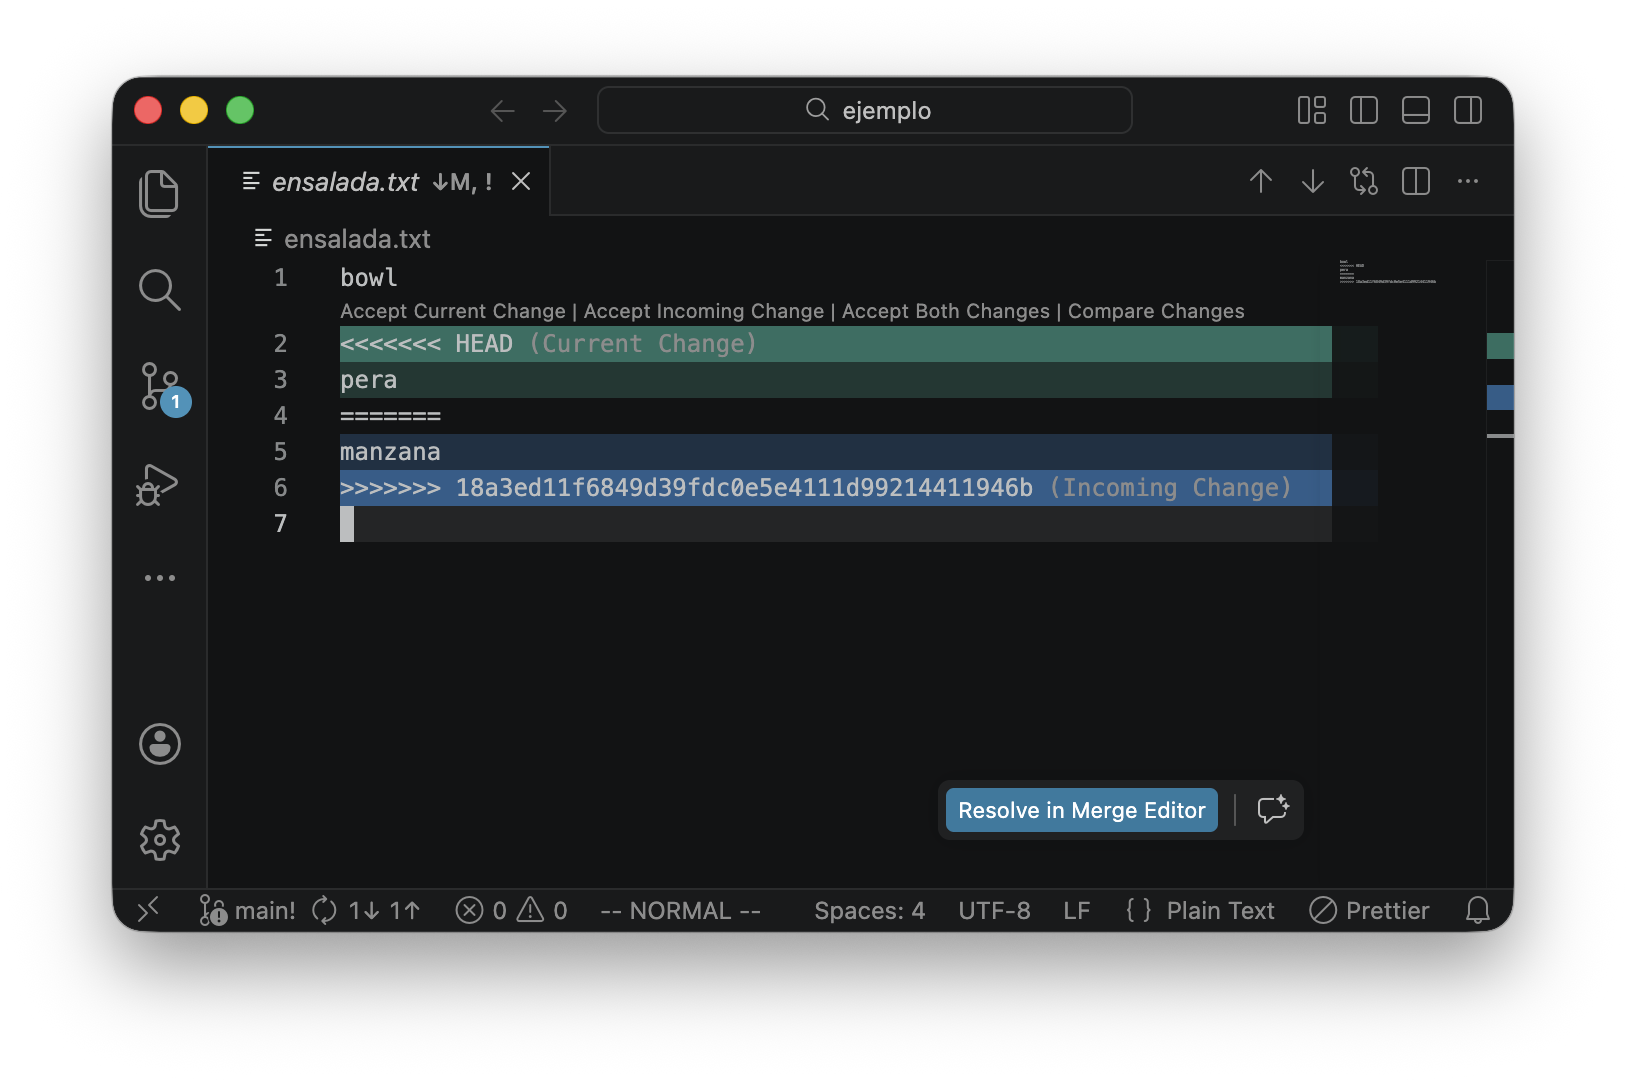
\includegraphics[height=2.4in]{images/vscode-conflict.png}
    \end{figure}
\end{frame}


\begin{frame}[t, fragile=singleslide]{... una vez ya resueltos}
    \begin{figure}[ht]
        \small
        \begin{Verbatim}[commandchars=\\\{\}]
\prompt{git add ensalada.txt}
\prompt{git commit -m "unificar ensaladas"}
[main 64a1772] unificar ensaladas
\prompt{git push}
Enumerating objects: 1, done.
Counting objects: 100% (1/1), done.
Writing objects: 100% (1/1), 427 bytes | 427.00 KiB/s, done.
Total 1 (delta 0), reused 0 (delta 0), pack-reused 0 (from 0)
To https://git.cubawiki.com.ar/mlang/ejemplo
   18a3ed1..821a6d8  main -> main
        \end{Verbatim}
    \end{figure}
\end{frame}

\begin{frame}[t]{Muy importante (?)}
    \begin{figure}[ht]
        \begin{center}
            
\includegraphics[height=2.6in]{images/in-case-of-fire.jpg}
        \end{center}
    \end{figure}
\end{frame}
